\documentclass[]{article}   % list options between brackets
\usepackage{graphicx} % Required to insert images
\usepackage{listings} % Required for insertion of code
\usepackage{courier} % Required for the courier font
\usepackage{amsmath}
\usepackage{enumitem}
\usepackage{subfigure}
\usepackage{float}
\usepackage{url}
\usepackage{authblk}
% type user-defined commands here

\title{Description of the project BrainActivity3D}   % type title between braces
\author{Anna Leontyeva, Ilya Kuzovkin and Dmytro Fishman} 

\affil{University of Tartu, Institute of Computer Science}


\begin{document}

         % type author(s) between braces

\maketitle
     
\section{Introduction}
BrainActivity3D is a graphical application that aims to visualize sources of a brain activity and allocate them inside the brain. It takes as an input electroencephalography (EEG) signal, applies signal processing and outputs coordinates of the strongest signal that corresponds to a muscle activity. The result is showed on a 3d model of the human brain with the highlighted source position.         

\section{Input data for EEG signal}
The central neural system consists of neurons that respond to stimuli and transmit information over long distances. When  neurons are activated, it produces current that can be measured with EEG systems.
 
The computational neuroscience lab has at its disposal EEG device (\url{http://www.emotiv.com}). The device has 14 electrodes that measure electrical activity at 14 points on the surface of a human scull. The figure \ref{fig:epoc_placement} illustrates the position of the electrodes in 2D. 
The device records the signal from all electrodes  \emph{TODO: Ilya input about frequencies and measures}.
The resulting data serves as an input for the BrainActivity3D application. It can be used both in real time with the device installed on a human by sending data each 2 sec (TODO: Ilya confirm) from the device to the application or pre-recorded data can be used.
  
\begin{figure}[!h]
\begin{center}
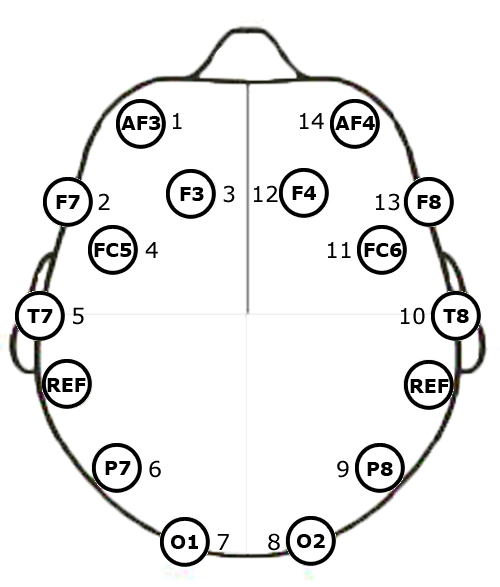
\includegraphics[width=0.5\columnwidth]{../Images/epoc_placement} 
\caption{}
\label{fig:epoc_placement}
\end{center}
\end{figure}
 
\section{Source localization techniques}
The main purpose of the application is to find the position of the activity sources inside the brain. It is not as straightforward as it seems: source localization is considered to be ill-defined. In order to provide an algorithm for localization of the sources within the brain, we need to make multiple assumptions. Firstly, we assume that source sends the electromagnetic wave to all 14 electrodes, thus, the strongest signal corresponds to the closest electrode. Secondly, we allocate fixed number of sources. \emph{TODO: Any other assumptions?}

We approach the problem of source localization using one of the method proposed by Zukov,L. et al \cite{zhukov2000}. To identify number of sources we perform Principal Component Analysis (PCA) and pick the number of components that describe $xx\%$ of the variance. Secondly, we perform Independent component analysis (ICA) to find the contributions of each source to each electrode. The contributions are then used to allocate the signal using penalized least-square optimization.

\section{Visualization aspects}
The application visualize a 3D model of the brain with differently colored lobes (see Figure \ref{fig:screenshot}). The brain can be displayed in two modes: solid one and completely transparent (use key \emph{'T'} to switch between two modes). Blue electrodes with corresponding labels are displayed slightly above the brain. The labels correspond to the conventional system $10-20$ recommended by the International Federation of Societies for Electroencephalography and Clinical Neurophysiology. illuminated source is positioned inside the brain. The lower corner provides constant information about the number of sources, the lobes, where they appear and the activity these lobes correspond to. The brain can be rotated (both with the mouse and the arrows of the keyboard) and zoomed (mouse). 
\begin{figure}[!h]
\begin{center}
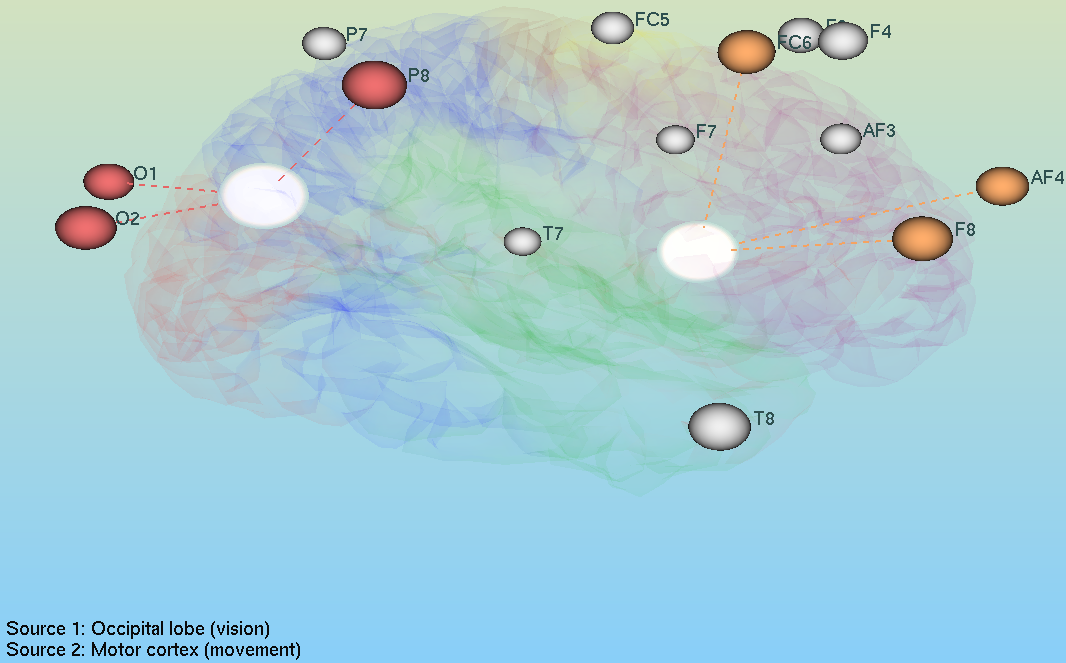
\includegraphics[width=1\columnwidth]{../Images/screenshot}
\caption{}
\label{fig:screenshot} 
\end{center}
\end{figure}

\section{Installation}
\emph{TODO Ilya}

\section{Example}
Let us take an example, how this application can be used. Position the device on a head of the subject according to the instructions provided with the device. Turn on the application and ask the patient to perform different activities (eye blinking, snapping teeth, thinking od something in particular). Follow the source moving in time from one position to another and compare it to the corresponding activity. If the subject blinks with right eyes, we expect the source to be on the right side in the frontal lobe near the electrode $F4$.  

\bibliographystyle{plain}
\bibliography{project_references}
 

\end{document}
